% \documentclass[english, draft]{article}
\documentclass[english]{article}

%\usepackage[showframe]{geometry}
\usepackage{geometry}
\usepackage{float}
\usepackage[utf8]{inputenc}
\usepackage[backend=biber,style= authoryear]{biblatex}
% \usepackage[backend=biber]{biblatex}
\usepackage[english]{babel}
\usepackage{csquotes}
% \usepackage[linktoc=none]{hyperref}
% \usepackage{hyperref}
\usepackage{graphicx}
\usepackage{subcaption}
\usepackage{booktabs}

% \usepackage{lipsum}
% Use more than one optional parameter in a new commands
\usepackage{xargs}
% Coloured text etc.
\usepackage[pdftex,dvipsnames,table]{xcolor}

\graphicspath{{./resources/images}}
\addbibresource{../articles.bib}
\addbibresource{../manual.bib}

\geometry{a4paper, total={165mm,257mm}, left=15mm, top=20mm,}

\def\changemargin#1#2{\list{}{\rightmargin#2\leftmargin#1}\item[]}
\let\endchangemargin=\endlist

\title{ Outline for \textit{Powdery Mildew} article}
\date{22nd July 2023}
\author{}

\begin{document}
\pagenumbering{arabic}
\maketitle

\begin{changemargin}{60pt}{60pt}
	\begin{abstract}
		TODO
	\end{abstract}
\end{changemargin}

\section*{Background}

\paragraph*{Powdery Mildew}

\begin{itemize}
	\item Description/taxonomy
	\item History \parencite*{fontaineEuropeBridgeheadWorldwide2021}
	\item Consequences
	      \begin{itemize}
		      \item Yield loss
		      \item Increased use of fongicides 80\% of usage for 20\% of area (\textbf{needs citation}) ->
		            \begin{itemize}
			            \item Increased costs
			            \item Ecological impact
			            \item Health impact
		            \end{itemize}
	      \end{itemize}
\end{itemize}

\paragraph*{Existing}

\begin{enumerate}
	\item Classical breeders -> poor quality wine
	\item Quality breeders \textbf{needs citation}
	\item Introduce OIV and OIV 452-1
	\item Critique scale \parencite{possamaiPhenotypingQTLIdentification2022}
	\item Manual Annotations
	\item Rpv3-, Rpv10- and Rpv12 \textbf{needs citation}
	\item Image processing tools \parencite{hernandezAssessmentDownyMildew2022}, \parencite{zendlerHighthroughputPhenotypingLeaf2021}
\end{enumerate}

\paragraph*{Novelty}

\begin{itemize}
	\item Current CV approaches only look at sporulation
	\item Our approach looks at sporulation 3 types of necrosis
	\item \textbf{TODO} \textbf{Goal}: Predict OIV 452-1 from images for binary variables
	\item \textbf{TODO} Test on existing experiments
\end{itemize}

\section*{Materials and Methods}

\subsection*{Plants}

\parencite{bellinResistancePlasmoparaViticola2009}

\subsection*{Infection}

\parencite{bellinResistancePlasmoparaViticola2009}

\subsection*{Image acquisition}

\begin{itemize}
	\item Acquisitions since 2018
	\item Multiple acquisition Methods
	\item Trays
\end{itemize}

\subsection*{Existing data overview}

\begin{figure}
	\begin{center}
		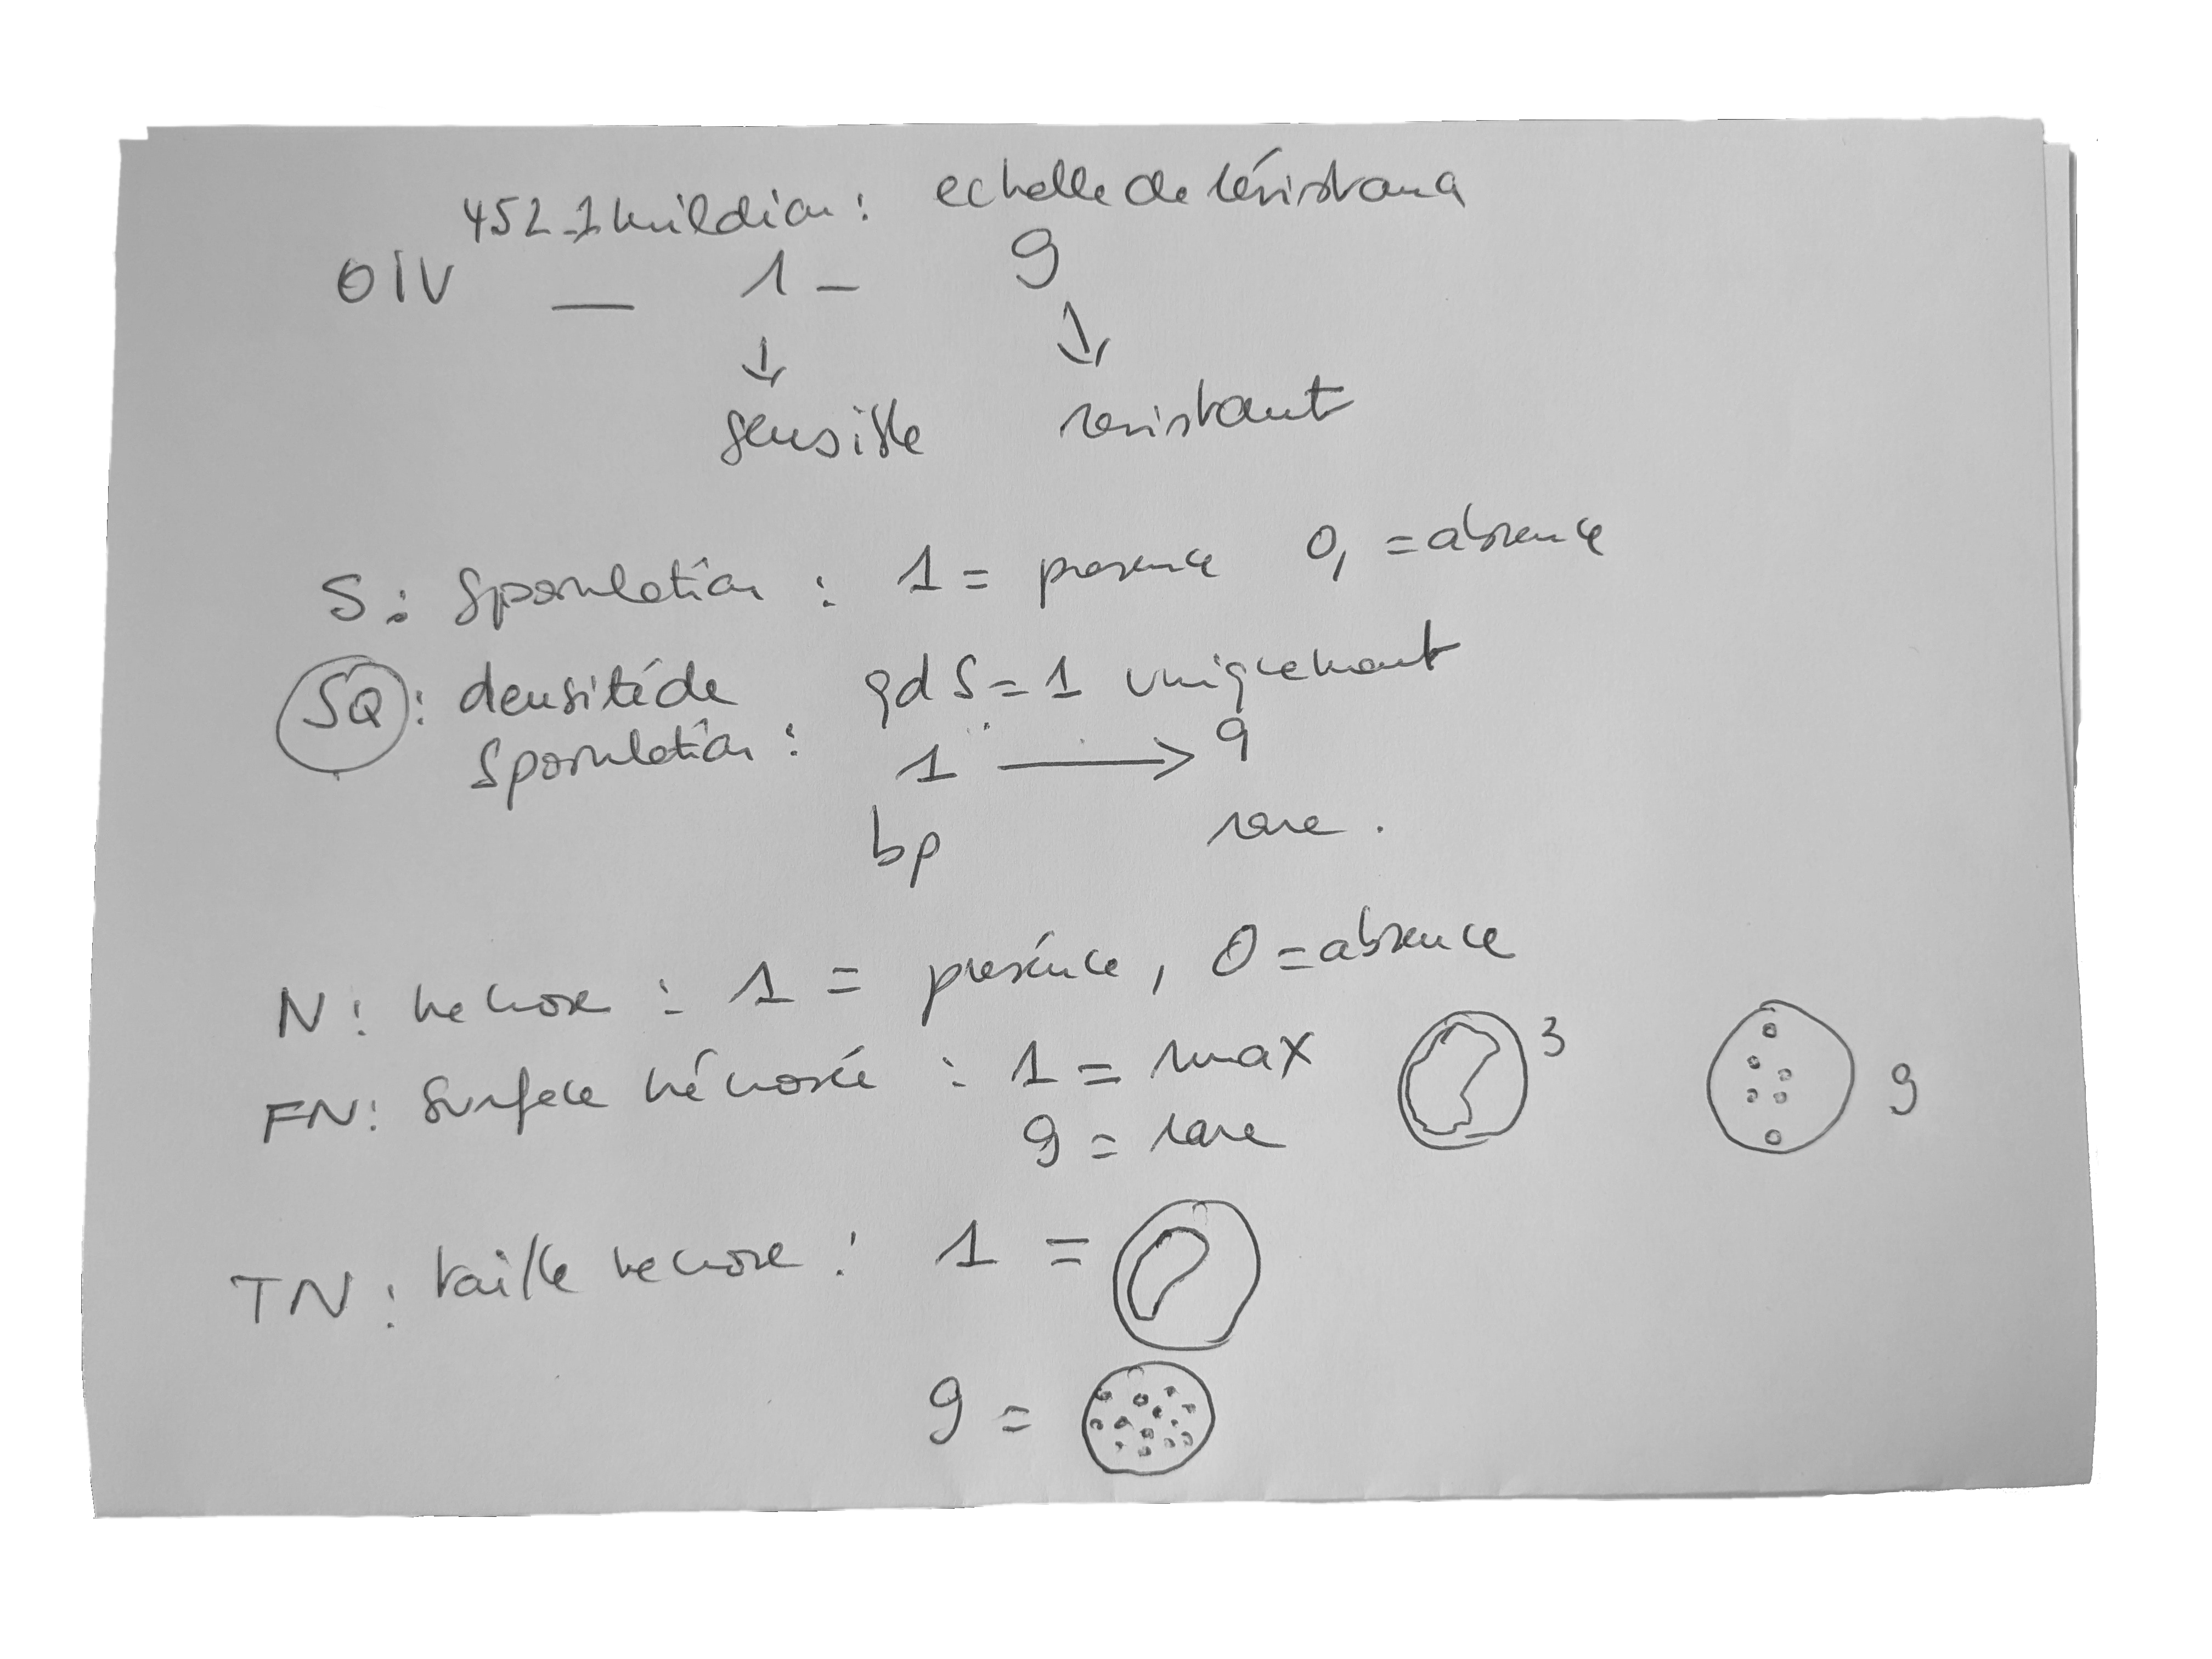
\includegraphics[width=0.7\linewidth]{oiv_452-1_desc.png}
		\caption{Additional variables}\label{fig:newvariables}
	\end{center}
\end{figure}

\begin{itemize}
	\item Images in folder
	\item OIV and additional variables
	      \begin{itemize}
		      \item OIV 452-1
		      \item New variables~\ref*{fig:newvariables}
	      \end{itemize}
	\item Excels
	\item -> Excel to CSV
	\item Naive prediction
	      \begin{itemize}
		      \item fail~\ref{fig:predictionfail}
		      \item multiple OIV values per combination~\ref*{tab:oivconfusion}
	      \end{itemize}
\end{itemize}

\begin{figure}[H]
	\begin{center}
		\includegraphics[width=0.7\linewidth,trim={1mm 0 0 0},clip]{annotations_da_rfc_cm.png}
		\caption{Prediction fail}\label{fig:predictionfail}
	\end{center}
\end{figure}

\begin{table}[H]
	\centering
	\caption{OIV row multi-value}\label{tab:oivconfusion}
	\begin{tabular}{rrrrrccccc}
		\toprule
		sporulation & sporulation & necrosis & necrosis & necrosis & oiv 1 & oiv 3 & oiv 5 & oiv 7 & oiv 9 \\
		{}          & density     & {}       & size     & area     & {}    & {}    & {}    & {}    & {}    \\
		\midrule
		1           & 1           & 0        & 1        & 1        & X     & X     & X     & X     &       \\
		1           & 7           & 1        & 3        & 5        & X     & X     & X     & X     &       \\
		1           & 5           & 1        & 9        & 9        & X     & X     & X     & X     &       \\
		1           & 5           & 1        & 1        & 7        &       &       & X     & X     &       \\
		1           & 1           & 1        & 3        & 1        &       &       & X     & X     &       \\
		0           & 1           & 1        & 3        & 3        &       &       &       & X     & X     \\
		\bottomrule
	\end{tabular}
\end{table}

\subsection*{Leaf Extraction}

\begin{itemize}
	\item Ilastik \parencite{bergIlastikInteractiveMachine2019}
	\item U-Net \parencite{ronnebergerUNetConvolutionalNetworks2015}
	\item Fast R-CNN \parencite{girshickFastRCNN2015}
	\item Indexation
\end{itemize}

\subsection*{Binary prediction}
Zooniverse \parencite{zooniverse}

\subsubsection*{Image Annotation}

\begin{figure}[H]
	\centering
	\begin{subfigure}[b]{0.2\linewidth}
		\includegraphics[width=\linewidth]{Exp21DM01_inoc1_T6_P24_c_2.png}
		\caption{Sporulation}\label{fig:sporulation}
	\end{subfigure}
	\begin{subfigure}[b]{0.2\linewidth}
		\includegraphics[width=\linewidth]{Exp20DM01_inoc1_T6_P17_c_1.png}
		\caption{Necrosis dots}\label{fig:necrosisdots}
	\end{subfigure}
	\begin{subfigure}[b]{0.2\linewidth}
		\includegraphics[width=\linewidth]{Exp20DM01_inoc2_T6_P47_c_4.png}
		\caption{Necrosis flecks}\label{fig:necrosisstains}
	\end{subfigure}
	\begin{subfigure}[b]{0.2\linewidth}
		\includegraphics[width=\linewidth]{Exp21DM01_inoc1_T6_P27_b_2.png}
		\caption{Necrosis senescence}\label{fig:necrosissenescence}
	\end{subfigure}
	\caption{The Four Phenotypes}\label{fig:phenotypes}
\end{figure}

Four phenotypes \ref*{fig:phenotypes}

\begin{table}[H]
	\caption{Zooniverse V1 data}\label{tab:zv1data}
	\begin{minipage}{0.4\linewidth}
		% \centering
		\caption{Class cardinals}\label{tab:zoonv1classcardinals}
		\begin{tabular}{rc}
			\toprule
			Phenotype           & Count \\
			\midrule
			sporulation         & 757   \\
			necrosis dots       & 247   \\
			necrosis flecks     & 149   \\
			necrosis senescence & 50    \\
			\bottomrule
		\end{tabular}
	\end{minipage}%
	\begin{minipage}{0.4\linewidth}
		\centering
		\caption{Classification report}\label{tab:zv1mcr}
		\begin{tabular}{rcccc}
			\toprule
			{}                                    & Precision & Recall & F1 score & Support \\
			\midrule
			sporulation                           & 0.92      & 0.93   & 0.93     & 113     \\
			necrosis dots                         & 0.82      & 0.38   & 0.52     & 37      \\
			\rowcolor{red!25} necrosis flecks     & 0.00      & 0.00   & 0.00     & 22      \\
			\rowcolor{red!25} necrosis senescence & 0.00      & 0.00   & 0.00     & 8       \\
			micro avg                             & 0.91      & 0.66   & 0.77     & 180     \\
			macro avg                             & 0.44      & 0.33   & 0.36     & 180     \\
			weighted avg                          & 0.75      & 0.66   & 0.69     & 180     \\
			\bottomrule
		\end{tabular}
	\end{minipage}
\end{table}

\begin{table}[H]
	\caption{Zooniverse V2 data}\label{tab:zv2data}
	\begin{minipage}{0.4\linewidth}
		\centering
		\caption{Class cardinals}\label{tab:zoonv2classcardinals}
		\begin{tabular}{rc}
			\toprule
			Phenotype           & Count \\
			\midrule
			sporulation         & 1188  \\
			necrosis dots       & 578   \\
			necrosis flecks     & 467   \\
			necrosis senescence & 271   \\
			\bottomrule
		\end{tabular}
	\end{minipage}%
	\begin{minipage}{0.4\linewidth}
		\centering
		\caption{Classification report}\label{tab:zv2mcr}
		\begin{tabular}{rcccc}
			\toprule
			{}                   & precision & recall & f1-score & support \\
			\midrule
			porulation           & 0.9922    & 0.9078 & 0.9481   & 141     \\
			necrosis\_dots       & 0.9388    & 0.8679 & 0.9020   & 106     \\
			necrosis\_stains     & 0.7313    & 0.7656 & 0.7481   & 64      \\
			necrosis\_senescence & 0.6800    & 0.8947 & 0.7727   & 38      \\
			micro avg            & 0.8808    & 0.8682 & 0.8745   & 349     \\
			macro avg            & 0.8356    & 0.8590 & 0.8427   & 349     \\
			weighted avg         & 0.8942    & 0.8682 & 0.8783   & 349     \\
			\bottomrule
		\end{tabular}
	\end{minipage}
\end{table}

\begin{itemize}
	\item round 1 -> class cardinal problems~\ref*{tab:zv1data}
	\item round 2 and + -> annotation conflict problems~\ref*{tab:zv2data}
	\item round 3 -> experts only. annotation by agreemment
\end{itemize}

\subsubsection*{OIV 452-1 prediction}

\subsection*{Experiments re-analysis}

\section*{Results}

\subsection{Unreliable human factor}

\section*{Discussion}

% \clearpage
\printbibliography

\end{document}

